\newcommand{\mvec}[1]{\mathbf{#1}}
\newcommand{\mvecx}[1]{\mathbf{#1}_x}
\newcommand{\mvecy}[1]{\mathbf{#1}_y}
\newcommand{\mvecz}[1]{\mathbf{#1}_z}
\newcommand{\mvecw}[1]{\mathbf{#1}_w}
\newcommand{\mmat}[1]{\mathbf{#1}}
\newcommand{\transpose}[1]{#1^{\mathsf{T}}}
\newcommand{\inverse}[1]{#1^{\mathsf{-1}}}
\newcommand{\normalise}[1]{\frac{#1}{\norm{#1}}}

\DeclarePairedDelimiter\abs{\lvert}{\rvert}
\DeclarePairedDelimiter\norm{\lVert}{\rVert}

%\renewcommand\Re{\operatorname{Re}}
%\renewcommand\Im{\operatorname{Im}}

\renewcommand{\Re}{\mathcal{R}}
\renewcommand{\Im}{\mathcal{I}} 

\begin{table}[b]
\begin{tabularx}{\textwidth}{X | X X | X X }
 %\hline
  \cline{2-5}
  & \multicolumn{2}{c}{Period Band Range (sec)} \vline & \multicolumn{2}{c}{Frequency Band Range (Hz)} \\
  \hline
  Wave Type & Start & End & Start & End \\
 \hline
  Capillary    & $0$                & $1\times10^{-1}$   & $\infty$            & $1\times10^1$ \\
  Ultragravity & $1\times10^{-1}$   & $1\times10^{0}$    & $1\times10^1$       & $1\times10^0$ \\
  Gravity      & $1\times10^{0}$    & $3\times10^{1}$    & $1\times10^0$       & $3.33\times10^{-2}$ \\
  Infragravity & $3\times10^{1}$    & $3\times10^{2}$    & $3.33\times10^{-2}$ & $3.33\times10^{-3}$ \\
  Long Period  & $3\times10^{2}$    & $8.64\times10^{4}$ & $3.33\times10^{-3}$ & $1.16\times10^{-5}$ \\
  Transtidal   & $8.64\times10^{4}$ & $\infty$           & $1.16\times10^{-5}$ & $0$
\end{tabularx}
\caption{A classification of ocean surface waves by period and frequency.}
\label{tab:ocean_wave_period}
\end{table}

Ocean surface waves are generated by different kinds of forces, such as storms, earthquakes,
the gravity of sun and moon, but with~\emph{wind} being the most prominent one.
Table~\ref{tab:ocean_wave_period} gives a compact overview of different kinds of ocean surface waves
classified by frequency. Figure~\ref{fig:surface_waves_energy}, inspired by Munk~\cite{article:munkorigin}
and Kinsman~\cite{book:kinsman2002wind}, on the other hand, pictures the forces
influencing them.\\

Because ocean surface waves are generated and propagate at the interface between the atmosphere
and the ocean, where the restoring force of gravity is in effect, they are classified as~\emph{surface gravity waves}.
Moreover, since wind blowing over a vast stretch of the air-sea interface is the main force to generate waves on
the ocean surface, this kind of waves is called~\emph{wind generated waves},
or in short,~\emph{wind waves}. Wind waves on the ocean surface represent
gravity waves, while e.g. tsunamis and ocean tides do not.\\

The process behind surface gravity waves is a simple one - the moment a fluid element at the interface is displaced, gravity
will try to restore it to equilibrium which results in oscillation of said fluid element. We mentioned before
that wind is the most prominent force causing displacement on the water surface. As it blows, it causes pressure and friction
forces which perturb the water surface's equilibrium. Therefore, the combination of wind transferring energy from the air
to the water and gravitational acceleration cause the formation of waves on the water surface.\\

In order to be able to model the surface of such an intricate fluid system as the ocean, one has to reduce complexity.
Research fields such as ocean engineering or coastal engineering employ the~\emph{Airy wave theory}\cite{book:airy1845tides}
to model the properties of the sea. Airy wave theory, also known as~\emph{linear wave theory}, describes the propagation of
gravity waves on the surface of a homogeneous fluid with a set of~\emph{linear} equations. These equations give
a decent approximation of the wave dynamics and kinematics with enough accuracy to model the state of the sea over a
limited amount of time.

\begin{figure}[tb]
	\centering
	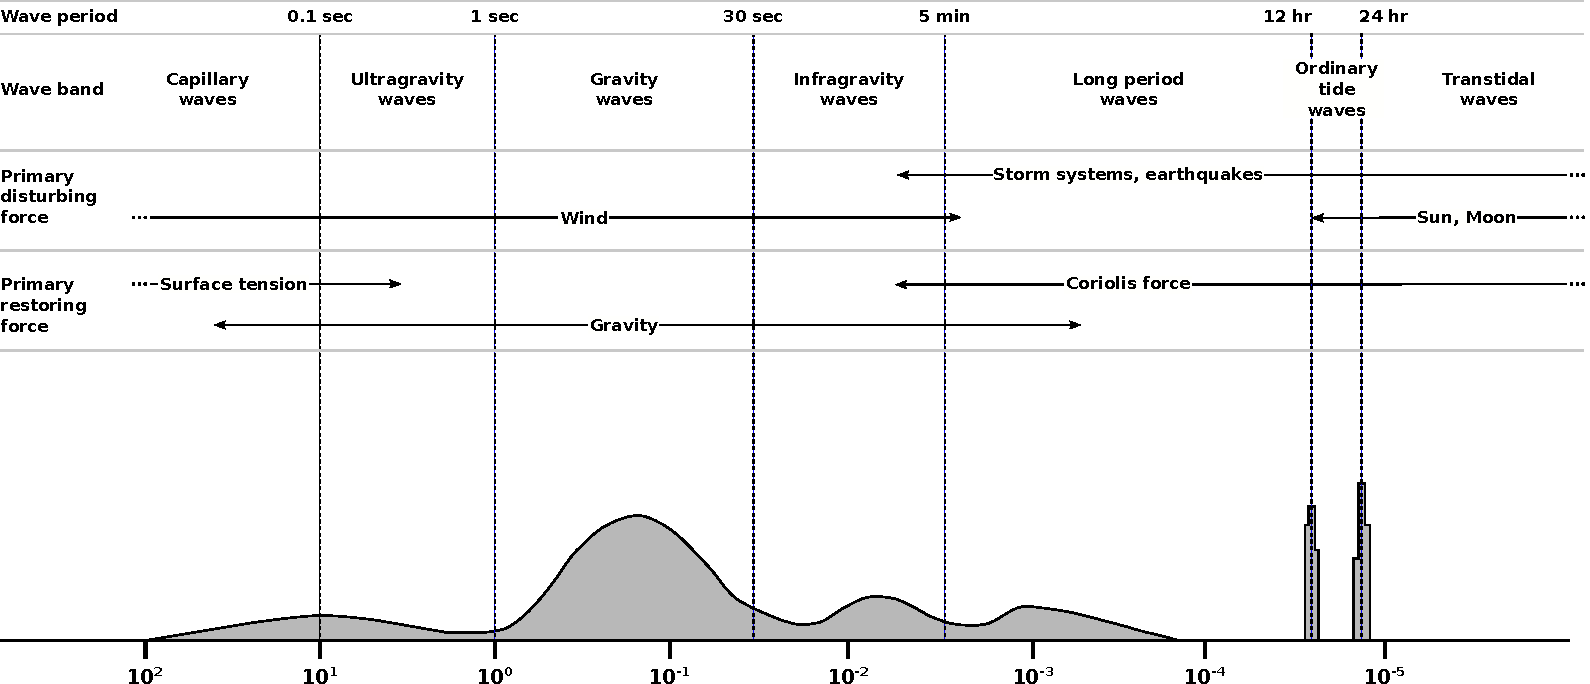
\includegraphics[width=\textwidth]{figures/SurfaceWavesEnergy}
	\caption{A tentative overview of which forces influence which wave band, as well as the relative amount of energy
each wave band contains.}
	\label{fig:surface_waves_energy}
\end{figure}

\section{Linear Theory of Ocean Surface Waves}
\label{sec:linear_theory_ocean_waves}
Linear wave theory makes a set of assumptions about the properties of the fluid, such as its viscosity,
compressibility and curl. Because fluid mechanics and fluid dynamics, associated fluid properties, and the derivation
of the linear wave theory go beyond the scope of this thesis, we will refer the interested reader
to Airy~\cite{book:airy1845tides}, Batchelor~\cite{book:batchelor2000introduction}
and Kinsman~\cite{book:kinsman2002wind}, which provide a good starting point for in-depth information.\\

\emph{But} we will mention two core assumptions of the linear wave theory which are easy to picture:
\begin{itemize}
 \item The water body has a uniform mean depth.
 \item The wave amplitudes are small in relation to the size of the water body.
\end{itemize}
Suppose we observe an idealized ocean in which exactly one sine wave is travelling constantly.
The parameters defining the sine wave - amplitude, frequency, length and direction - are all fixed.
To simplify the mathematics we assume a two-dimensional ocean, with one
dimension representing the wave's direction of travel and the  other the wave's
vertical displacement. With these assumptions we can describe surface elevation
as a sinusoid
%
\begin{equation}
\label{eq:sinusoid}
 \eta(x, t) = A\cos(kx - \omega t)\\
\end{equation}
with
\begin{align}
\label{eq:sinusoid_parameters}
 k &= \frac{2\pi}{\lambda} & \omega &= 2\pi f & f &= \frac{1}{T}
\end{align}
%
where $A$ is the amplitude, $k$ is called the~\emph{wave number},~$x$ is the horizontal position,
$\omega$ is the~\emph{wave frequency} in radians per second,~$t$ represents the time,
$\lambda$ is the~\emph{wave length},~$f$ is the~\emph{wave frequency} in Hertz (Hz) and~$T$
is the wave period in seconds.\\

\begin{figure}[b]
	\centering
	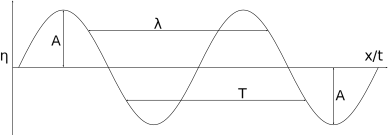
\includegraphics[width=\textwidth]{figures/sinusoid}
	\caption{An example of a sinusoidal wave.}
	\label{fig:sinusoid}
\end{figure}
%
We may picture Equation~\ref{eq:sinusoid} in an easy way if we either focus on a
fixed position $x$ or a fixed point in time $t$, see Figure~\ref{fig:sinusoid}.
If we assume a fixed position, we can see the surface elevation evolve through
time at that position. On the other hand, if we assume a fixed point in time, we
can observe surface elevation at all positions at that specific time. The wave's
high point is called a~\emph{crest}, its low point a~\emph{trough}. Because
surface elevation is described by a cosinus function, all crests and all troughs
will have the same elevation. Another effect of the cosinus function is that the
surface elevation is limited by the amplitude $A$. We will call the difference
in elevation between crest and trough the~\emph{wave height}. It is easy to see
that wave height $H$ is defined as follows:
\begin{equation}
 H = 2A
\end{equation}
\\

\subsection{Phase Velocity}
\label{sec:phase_velocity}
In linear wave theory, the rate at which a particular phase of a wave propagates in space is called
the~\emph{phase velocity}. The phase velocity is a vector and has an associated direction,
the \emph{phase speed} on the other hand refers only to the magnitude of the phase velocity.
The most comprehensible example of phase speed is the rate of propagation of the wave crest.
During one wave period $T$ the wave crest travels a distance equal to the wave length $\lambda$.
We may generalize this to other phases than the wave crest - given a constant phase
\begin{equation}
  const = kx - \omega t
\end{equation}
the surface elevation $\eta$ will always be the same. We rewrite the term to
\begin{equation}
  x = \frac{\omega}{k}t + \frac{const}{k}
\end{equation}
which gives us all positions $x$ the wave has the same value at. These positions are time dependent,
differentiation gives us phase speed $c$:
\begin{equation}
  c = \frac{\mathrm dx}{\mathrm dt} = \frac{\lambda}{T} = \frac{\omega}{k}
\end{equation}

\subsection{The Dispersion Relation}
\label{sec:dispersion_relation}

In the context of water surface waves,~\emph{dispersion} refers to~\emph{frequency dispersion}, which describes
the effect of waves at different wavelengths travelling at different phase speeds. We have seen that
phase speed $c = \frac{\lambda}{T}$ involves wave length and frequency, and alternatively $c = \frac{\omega}{k}$
which includes angular frequency and wave number. We focus on the latter formulation for phase speed, because
linear wave theory defines a functional relationship between the two factors involved:
%therefore we will start with the functional relationship
%between angular frequency~$\omega$ and wave number~$k$ as defined by linear wave theory:
\begin{equation}
\label{eq:dispersion_relation}
 \omega^2 = gk\tanh(kd)
\end{equation}
%
where $g$ is the acceleration of earth's gravity and $d$ is the water depth. Equation~\ref{eq:dispersion_relation}
is called the~\emph{dispersion relation}.\\

There exist two useful approximations of Equation~\ref{eq:dispersion_relation} which do not involve the $\tanh$ term:
\begin{itemize}
 \item \emph{Shallow water approximation} - the water depth $d$ is much smaller than the wave length $\lambda$.
 Assume $d \ll \lambda$, then $0 \leq kd \ll 1$ and $\tanh(kd) \approx kd$.
 \item \emph{Deep water approximation} - the water depth $d$ is much larger than the wave length $\lambda$.
 Assume $d \gg \lambda$, then $kd \gg 1$ and $\tanh(kd) \approx 1$.
\end{itemize}
%
The reduced dispersion relations are as follows:
\begin{align}
\label{eq:disp_rel_shallow_water}
\omega^2 & = gk^2d && \text{with} & d &< \frac{\lambda}{20}  && \text{Shallow 
water dispersion relation}\\
\label{eq:disp_rel_deep_water}
\omega^2 & = gk    && \text{with} & d &> \frac{\lambda}{2} && \text{Deep water 
dispersion relation}
\end{align}
%
Given the dispersion relation approximations for shallow and deep water, the corresponding
phase speeds are:
\begin{align}
 \label{eq:phase_speed_shallow_water} c &= \sqrt{gd} && \text{Shallow water phase speed}\\
  \label{eq:phase_speed_deep_water}   c &= \sqrt{\frac{g}{k}} = \frac{g}{\omega} && \text{Deep water phase speed}
\end{align}
%
According to Equation~\ref{eq:phase_speed_shallow_water}, in shallow water phase speed depends exclusively
on water depth and gravitational acceleration, there is no connection to wave length or frequency.
We may conclude that waves with different wave lengths travel with the same phase speed, it follows that
~\emph{shallow water is not dispersive}. Phase speed in deep water, on the other hand,
does not relate to water depth, but to wave length and frequency, which makes~\emph{deep water dispersive}.
We can expand Equation~\ref{eq:phase_speed_deep_water} to:
%
\begin{equation}
\label{eq:phase_speed_deep_water_l}
 c = \sqrt{\frac{g\lambda}{2\pi}} = \frac{gT}{2\pi}
\end{equation}
%
Looking at Equation~\ref{eq:phase_speed_deep_water_l} we can conclude that phase speed in deep water increases
with wave length $\lambda$ ~\emph{and} with wave period $T$. Waves in deep water with large wavelengths/periods
travel faster than those with smaller ones.
%
\subsection{Three Dimensional Wave}
Until now we were discussing a two dimensional ocean defined by exactly one sinus wave. As a first
step to get to a more realistic ocean surface representation we will extend equation~\ref{eq:sinusoid}
to form a wave in three dimensional space. In contrast to equation~\ref{eq:sinusoid}, where the wave's
travelling direction is fixed, the wave has to be able to travel in an arbitrary direction on a plane.
Moreover, we need to handle two dimensional input positions. The sinusoid describing surface elevation
in three dimensional space is defined as follows:
\begin{equation}
\label{eq:sinusoid_3d}
 \eta(\mvec{x}, t) = A\cos(\transpose{\mvec{k}}\mvec{x} - \omega t)
\end{equation}
where $\mvec{x} = (x_x, x_z)$ denotes the observed point on a plane and $\mvec{k} = (k_x, k_z)$ represents
the travelling direction of the wave. The wave number $k$ of~\emph{wave vector} $\mvec{k}$ is determined by
the wave vector's magnitude
\begin{equation}
 k = \norm{\mvec{k}}
\end{equation}
Thus, because of the dispersion relation, all waves of same magnitude share the same frequency.

\subsection{Sum of Waves}
Now that we have a description of waves in three-dimensional space, we need to
enhance the description of the ocean surface. It is obvious that the ocean does
not consist of only one wave travelling, but of an infinite number of waves with
different lengths and directions. Because we find ourselves still in the realm
of~\emph{linear} wave theory, we may reach an adequate solution
by~\emph{combination}. A linear combination of solutions constitutes a valid
solution as well.\\

Before we start handling a large number of sinusoids, we will improve our
notation to make it more compact. In order to do that we employ~\emph{Euler's
formula}\fxerror{Reference}:
\begin{align}
\label{eq:euler_positive} e^{ix} &= \cos{x} + i\sin{x} && x \in \mathbb{R} \\
\label{eq:euler_negative} e^{-ix} &= \cos{x} - i\sin{x} && x \in \mathbb{R}
\end{align}
%
We may extract both the real and the imaginary part separately:
\begin{align*}
 \cos{x} &= \Re\{e^{ix}\} \\
 \sin{x} &= \Im\{e^{ix}\}
\end{align*}
where $\Re$ denotes the real part of the exponential and $\Im$ the
complex one. Alternatively we may solve Equations~\ref{eq:euler_positive}
and~\ref{eq:euler_negative} as a pair in the variables $\cos{x}$ and $\sin{x}$
\begin{align*}
 \cos{x} &= \frac{e^{ix}+e^{-ix}}{2}\\
 \sin{x} &= \frac{e^{ix}-e^{-ix}}{2i}\\
\end{align*}
Now we are able to rewrite our current formulation of a sinusoid in three
dimensional space from Equation~\ref{eq:sinusoid_3d} as an exponential:
%
\begin{align}
\label{eq:sinusoid_exponential_sa} \eta(\mvec{x}, t) &=
\Re\{A\mathrm{e}^{\mathrm{i}[\transpose{\mvec{k}}\mvec{x} -{\omega}t]}\} \\
\intertext{or equivalent}
 p &= A\mathrm{e}^{\mathrm{i}[\transpose{\mvec{k}}\mvec{x} -
{\omega}t]} \\
 \eta(\mvec{x}, t) &= \frac{p+p^*}{2}
\end{align}
%
where $p^*$ denotes the~\emph{complex conjugate} of $p$. From now on we will
omit the explicit $\Re$ in equations expressing $\eta$, because surface
elevation is a real number.\\

Each combination of amplitude $A$, wave vector $\mvec{k}$ and wave frequency
$\omega$ identifies one particular wave. As a next step we get rid of the
restriction of one single amplitude $A$ for all wave components. We replace the
constant amplitude $A$ with $a(\mvec{k})$ in order to create a dependency
between wave vector and wave amplitude. Furthermore, because of the dispersion
relation, we can express frequency as a function of the wave vector, $\omega =
\omega(\mvec{k})$. Now we are able to rewrite
Equation~\ref{eq:sinusoid_exponential_sa} as follows:
\begin{equation}
\label{eq:sinusoid_exponential_ak_wk}
\eta(\mvec{x}, t) =
a(\mvec{k})\mathrm{e}^{\mathrm{i}(\transpose{\mvec{k}}\mvec{x}-
\omega(\mvec{k})t)}
\end{equation}
%
We already mentioned that we seek a solution by linear combination. Armed with
Equation~\ref{eq:sinusoid_exponential_ak_wk} we may express surface
elevation as an infinite sum of sinusoids:
\begin{equation}
\label{eq:surface_elevation_akwt}
 \eta(\mvec{x}, t) = \int_{\mvec{k}}
a(\mvec{k})~\mathrm{e}^{\mathrm{i}(\transpose{\mvec{k}}\mvec{x}-
\omega(\mvec{k})t)}~\mathrm{d}\mvec{k}
\end{equation}
where $a(\mvec{k})$ is called the~\emph{amplitude spectrum} of
$\eta(\mvec{x}, t)$. According to Kinsman~\cite{book:kinsman2002wind} it is possible to
represent the vertical displacement of the water surface by~\emph{Generalized
Fourier Transforms}. We may write the sea surface in two spatial dimensions and
one time dimension as
%
\begin{equation}
\label{eq:surface_elevation_bkwt}
 \eta(\mvec{x}, t) = \iint_{\mvec{k}}\int_{\omega} B(\mvec{k},
\omega)~\mathrm{e}^{\mathrm{i}(\transpose{\mvec{k}}\mvec{x}-
\omega t)}~
\mathrm{d}\mvec{k}~\mathrm{d}\omega
\end{equation}
where the $\mvec{k}$ integration is over all wave-number space and the $\omega$
integration is over all frequencies. $B(\mvec{k},\omega)$ is called the
three dimensional amplitude spectrum of $\eta(\mvec{x}, t)$. Notice the missing
dependency of $\omega$ on $\mvec{k}$ in the exponent, it is the responsibility
of $B(\mvec{k},\omega)$ to model that relationship.\\

We may integrate separately over all frequencies
%
\begin{equation}
 B(\mvec{k}, t) = \int_{\omega} B(\mvec{k},
\omega)~\mathrm{e}^{-\mathrm{i}\omega t}~\mathrm{d}\omega
\end{equation}
to obtain the two dimensional amplitude spectrum $B(\mvec{k}, t)$. We rewrite
Equation~\ref{eq:surface_elevation_bkwt} as
\begin{equation}
\label{eq:surface_elevation_bk}
 \eta(\mvec{x}, t) = \iint_{\mvec{k}} B(\mvec{k},t)
~\mathrm{e}^{\mathrm{i}\transpose{\mvec{k}}\mvec{x}}~
\mathrm{d}\mvec{k}
\end{equation}
%
Alternatively, we may integrate over all wave numbers
\begin{equation}
 B(\mvec{x}, \omega) = \iint_{\mvec{k}} B(\mvec{k},
\omega)~\mathrm{e}^{\mathrm{i}\transpose{\mvec{k}}\mvec{x}}~\mathrm{d}\mvec{k}
\end{equation}
%
to obtain the one dimensional amplitude spectrum $B(\mvec{x}, \omega)$. We
rewrite Equation~\ref{eq:surface_elevation_bkwt} as
\begin{equation}
\label{eq:surface_elevation_bw}
\eta(\mvec{x}, t) = \int_{\omega} B(\mvec{x},\omega)
~\mathrm{e}^{-\mathrm{i}\omega t}~\mathrm{d}\omega
\end{equation}
%
\section{The Specification of a Random Sea}
\label{sec:random_sea}
%
Equation~\ref{eq:surface_elevation_bk} may be able to describe the ocean
surface, but at the cost of deducing an amplitude spectrum for each observed
point on the sea surface, which poses a both tedious and unfeasible task. At
this point we are in need of a general description of $B$ which is valid at all
points $\mvec{x}$ and times $t$. Fortunately, modern physical oceanography is
based on exactly such a formulation, which has been developed in the 1950s
by~\emph{Pierson} and~\emph{von Neumann}. \fxerror{References} We will refer to
said formulation as~\emph{Pierson-Neumann theory} throughout the remainder of
this document.\\

Pierson and von Neumann combine oceanography, physics and stochastics in order
to describe the ocean surface. A fundamental assumption of their theory is that
surface disturbance is formed from many contributions caused by relatively
unrelated forces at different times. Therefore it is reasonable to presume that
the elements in the summation of Equation~\ref{eq:surface_elevation_bk} are
statistically independent. As a consequence the central limit theorem with the
resulting distribution being a Gaussian is applied. The result is
a~\emph{spatially homogeneous} and~\emph{temporally stationary} gaussian random
process which models a wind driven ocean surface. The process is said to be
\emph{homogeneous}, because it is independent of the origin selected for
positions $\mvec{x}$, futhermore it is~\emph{stationary} since absolute time is
irrelevant, only time differences matter.
%
\subsection{The Energy Spectrum}
\label{sec:energy_spectrum}
Given a spatially homogeneous and temporally stationary wave field, and a
respective three dimensional amplitude spectrum $B(\mvec{k},\omega)$, then we
may write
\begin{equation}
\label{eq:energy_spectrum_3d}
 \Theta(\mvec{k}, \omega) = \frac{B(\mvec{k}, \omega)^2}{2} = 
\overline{B(\mvec{k}, \omega)B^{*}(\mvec{k}, \omega)}
\end{equation}
where the $\overline{B}$ operator denotes the mean and
$\Theta(\mvec{k},\omega)$ represents the~\emph{mean square displacement} of
wave amplitude $B(\mvec{k},\omega)$. The mean square displacement of a wave
is connected to wave energy $E_w$ as follows:
%
\begin{equation}
\label{eq:wave_energy_single}
 E_w = \rho g~\Theta(\mvec{k},\omega)
\end{equation}
%
where $\rho$ is the water density and $g$ the accleration of earth's gravity.
Equation~\ref{eq:wave_energy_single} is the reason $\Theta(\mvec{k},\omega)$
in literature is referred to as the three dimensional~\emph{energy spectrum}
associated with $B(\mvec{k},\omega)$. Now we are able to define mean surface
energy $E_s$ based on combined wave energy:
%
\begin{equation}
\label{eq:wave_energy_3d}
 E_s = \rho g~\iint_{\mvec{k}}\int_{\omega}\Theta(\mvec{k},\omega)
~\mathrm{d}\mvec{k}~\mathrm{ d}\omega
\end{equation}
%
Looking back at Equation~\ref{eq:wave_energy_single}, which makes wave energy
dependent on the mean square displacement of wave amplitudes, we may deduce that
mean surface energy is dependent on the~\emph{mean square surface displacement},
denoted as $\overline{\eta^2}$. Therefore, we may write:
%
\begin{equation}
\label{eq:mean_square_eta}
\overline{\eta^2} = \iint_{\mvec{k}}\int_{\omega}\Theta(\mvec{k},\omega)
~\mathrm{d}\mvec{k}~\mathrm{d}\omega
\end{equation}
%
\\
Later on we will be in need of energy spectrum formulations which have a lower
dimensionality than the three dimensional $\Theta(\mvec{k},\omega)$. As such,
we introduce the two dimensional energy spectrum, in literature known
as~\emph{wave number spectrum}, which is as follows:
\begin{equation}
\label{eq:energy_spectrum_2d}
 \Theta(\mvec{k}) = \int_{\omega} \Theta(\mvec{k}, \omega)~\mathrm{d}\omega
\end{equation}
The wave number spectrum gives the contribution to the wave energy arising from
wave components with wave number $k$ dependent on wave vector $\mvec{k}$,
irrespective of the frequencies $\omega$ associated with that wave number. In
contrast, the one dimensional energy spectrum, in literature known
as~\emph{frequency spectrum}, is defined as follows:
\begin{equation}
\label{eq:energy_spectrum_1d}
 \Theta(\omega) = \int_{\mvec{k}} \Theta(\mvec{k}, \omega)~\mathrm{d}\mvec{k}
\end{equation}
The frequency spectrum gives the contributions to the energy coming from each
frequency $\omega$, irrespective of the wave numbers associated with that
frequency.\\

The energy spectrum $\Theta$ as presented is severely restricted in its
capabilities to model a~\emph{dynamic} ocean. Dynamic, in this context, means an
ocean which may start as a perfectly flat surface, is actuated to a fully
developed sea by wind, decays back into a near motionless state, and so on and
so forth. The energy spectrum discussed models waves on an ocean with infinite
extend over which a uniform wind has been blowing forever. In context of this
document such a model of the ocean is sufficient, there is no need to simulate
the actual generation and decay of waves over time.

\subsection{The Random Process}
\label{sec:random_process}
Pierson-Neumann theory describes the sea surface as a gaussian random process.
As such, we are not dealing with one concrete ocean surface $\eta$, but with an
\emph{ensemble} of different sea surfaces $\{\eta\}$, each associated with its
own probabilty to be actually realised. Because the random process is a
gaussian one, it has an associated gaussian distribution with mean
$\mathrm{E}[\eta]$ and variance $\mathrm{Var}[\eta] = \sigma^2$. Considering a
sea surface in combination with linear wave theory, where a symmetry between
troughs and crests is a given, the mean is easily found
\begin{equation}
 \mathrm{E}[\eta] = 0
\end{equation}
%
Moreover, all spectral components $B(\mvec{k},\omega)$ are assumed to be
\emph{statistically independent}, each with mean zero and variance $\Theta(\mvec{k},\omega)$,
therefore the variance of all components combined is
\begin{equation}
\label{eq:random_process_variance}
\mathrm{Var}[\eta] = \sigma^2 = \iint_{\mvec{k}}
\int_{\omega}\Theta(\mvec{k},\omega)~\mathrm{d}\mvec{k}~\mathrm{ d}\omega
\end{equation}
which is the same as Equation~\ref{eq:mean_square_eta}. The variance
$\sigma^2$ is equal the mean square surface elevation $\overline{\eta^2}$. With
mean and variance in our hands, we may write the gaussian distribution that the
values of sea surface elevation are drawn from, as follows:
\begin{equation}
\label{eq:gaussian_dist}
 pr[\eta] = \frac{1}{\sqrt{2\pi E}}~\mathrm{e}^{-\frac{\eta^2}{2E}}
\end{equation}
Note that neither position nor time appear in the distribution, because the
process is modeled as spatially and temporally invariant.\\

We already mentioned that Pierson-Neumann theory does not represent surface
elevation $\eta$ as one single function, but as an ensemble of functions
$\{\eta\}$. The ensemble contains an infinite number of different sea surfaces,
each with its own probability of actually being realised. As of now, we may
formulate surface elevation as a realisation of a stochastic process
\begin{equation}
\label{eq:surface_elevation_gauss}
 \eta(\mvec{x}, t) = \iint_{\mvec{k}}\int_{\omega} \xi
~\mathrm{e}^{\mathrm{i}(\transpose{\mvec{k}}\mvec{x}-
\omega t)}~
\mathrm{d}\mvec{k}~\mathrm{d}\omega
\end{equation}
where $\xi$ is a gauss distributed variable with mean $\mathrm{E}[\eta] = 0$ and
variance $\mathrm{Var}[\eta] = \sigma^2$ defined by the energy spectrum
$\Theta(\mvec{k}, \omega)$. One may realize that in context of this formulation
of sea surface elevation, the energy spectrum $\Theta$ is the key to believable
ocean surfaces, as it needs to be able to model the underlying physical
processes to give realistic results.\\

At this point we have to face the reality of oceanographic research, which does 
not provide us with any three dimensional energy spectra 
$\Theta(\mvec{k},\omega)$. On the other hand, we are given a set of 
parametric one dimensional frequency spectra $\Theta(\omega)$ which we are not 
able to use as-is, because they do not contain any information about the 
travelling direction of waves, and therefore are not able to simulate 
surface elevation with two dimensional positions $\mvec{x}$ as input. Hence, we 
have to settle for the two dimensional wave number spectrum $\Theta(\mvec{k})$ 
as basis from which we will compute surface elevation. We write surface 
elevation as follows:
\begin{equation}
\label{eq:surface_elevation_gauss_2d}
 \eta(\mvec{x}, t) = \iint_{\mvec{k}} 
\xi~\mathrm{e}^{-\mathrm{i}\omega(\mvec{k}) t}
~\mathrm{e}^{\mathrm{i}\transpose{\mvec{k}}\mvec{x}}~\mathrm{d}\mvec{k}
\end{equation}
where, in lieu with Equation~\ref{eq:surface_elevation_gauss}, $\xi$ is 
a gauss distributed variable with mean $\mathrm{E}[\eta] = 0$ and
variance $\mathrm{Var}[\eta] = \sigma^2$ defined by the energy spectrum
$\Theta(\mvec{k})$. Moreover, for animation purposes, we add the term 
$\mathrm{e}^{-\mathrm{i}\omega(\mvec{k}) t}$ in order to explicitely handle 
time $t$, because the two dimensional wave number spectrum has no notion of 
it. Equation~\ref{eq:surface_elevation_gauss_2d} represents a two dimensional 
\emph{inverse Fourier Transform} of Fourier components 
$\xi\mathrm{e}^{-\mathrm{i}\omega(\mvec{k}) t}$. For the remainder of the 
document, Equation~\ref{eq:surface_elevation_gauss_2d} will be the basis for all 
further discussions of specific wave spectrum models. Moreover, in 
Section~\ref{sec:1d_frequency_spectra} we will discuss the conversion of the 
more common one dimensional frequency spectra $\Theta(\omega)$ into two 
dimensional wave number spectra $\Theta(\mvec{k})$ for our practical usage.
%
\section{Discretisation}
For computer graphics applications we are in need of a discrete approximation 
of surface elevation as defined by 
Equation~\ref{eq:surface_elevation_gauss_2d}, 
which gives acceptable results as well as computes said results in a reasonable 
amount of time. We may write a rough sketch of such a discrete formulation like 
the following:
\begin{equation}
\label{eq:surface_elevation_sketch}
 \eta(\mvec{x}, t) = \sum_{\mvec{k}} 
\xi~\mathrm{e}^{-\mathrm{i}\omega(\mvec{k}) t}
~\mathrm{e}^{\mathrm{i}\transpose{\mvec{k}}\mvec{x}}
\end{equation}
Equation~\ref{eq:surface_elevation_sketch} represents a discrete inverse 
Fourier transform of Fourier components 
$\xi\mathrm{e}^{-\mathrm{i}\omega(\mvec{k}) t}$, which we are able to compute in 
a very efficient manner by means of the~\emph{Fast Fourier Transform}, 
~\emph{FFT} in short. The interested reader may find extensive discussions of 
the discrete Fourier transform and the Fast Fourier algorithm
in~\emph{Bracewell}\cite{book:bracewell2000fourier} 
and~\emph{Press}\cite{book:numericalrecipes}.\\

Employing the FFT algorithm may solve our concerns relating to performance, but 
we still have to make sure we compute an as good as possible approximation to 
Equation~\ref{eq:surface_elevation_gauss_2d}. Since our model for surface 
elevation is based on wave energy, the best way forward seems to be, that we 
choose a finite range of wave vectors $\mvec{k}$ such that they are 
representative of the whole energy $Var[\eta]$ defined by $\Theta(\mvec{k})$. 
Because wave vectors $\mvec{k}$ are related to wave length, they are also 
related to the spatial domain, and as such to positions $\mvec{x}$. Hence, the 
quality of our approximation depends on how we discretise both the spatial 
domain into a finite set of positions $\mvec{x}$ and the wave vector domain 
into a finite set of wave vectors $\mvec{k}$.
%
\subsection{Domain Discretisation}
\label{sec:domain_discretisation}
%
\begin{figure}
\centering
\begin{tikzpicture}
% let both axes use the same layers
\pgfplotsset{set layers}
\begin{axis}[
    grid=major,
    enlargelimits=false,
    scale only axis,
    axis equal=true,
%    width = \textwidth,
    xmin=-5,
    xmax=5,
    ymin=-5,
    ymax=5,
    xtick = {-4,0, 4},
    ytick = {-4,0, 4},
    xticklabels={$-\frac{N}{2}$,0,$\frac{N}{2}$},
    yticklabels={$-\frac{M}{2}$,0,$\frac{M}{2}$},
    xlabel={$\alpha$},
    ylabel={$\beta$},
    ]
\addplot graphics[
    xmin=-5,
    xmax=5,
    ymin=-5,
    ymax=5,
]
{figures/ifft_spatial_domain};
\end{axis}
%
\begin{axis}[
    enlargelimits=false,
    scale only axis,
    axis equal=true,
%    width = \textwidth,
    xmin=-5,
    xmax=5,
    axis x line* = top,
    ymin=-5,
    ymax=5,
    axis y line* = right,
    xtick = {-4,0, 4},
    ytick = {-4,0, 4},
    xticklabels={$-\frac{L}{2}$,0,$\frac{L}{2}$},
    yticklabels={$-\frac{K}{2}$,0,$\frac{K}{2}$},
    xlabel = {$\alpha\cdot\Delta x$},
    ylabel={$\beta\cdot\Delta y$},
    ]
\end{axis}
\end{tikzpicture}
\caption{The spatial domain in terms of index pairs $(\alpha,\beta)$ and
associated coordinate pairs $(\alpha\Delta x,\beta\Delta y)$.}
\label{fig:spatial_domain}
\end{figure}
%
We define the sea surface we want to synthesize as a rectangular area, with $L$
and $K$ denoting width and height in meters respectively. Moreover, we
discretise said rectangle into a grid with horizontal resolution $N$ and
vertical resolution $M$, where both $N$ and $M$ shall be an integer which can
be represented as a power of two. Therefore we will define sea surface elevation 
at $N\times M$ discrete points. We will denote the horizontal and vertical
distance between consecutive grid points as follows:
\begin{align}
 \Delta x = \frac{L}{N} && \Delta y = \frac{K}{M}
\end{align}
We will follow Tessendorf's lead~\cite{course:simulatingocean} and compute
surface elevation at the following points:
\begin{equation}
\label{eq:spatial_domain}
 \mvec{x} = (x,y)~\in~\{(\alpha\Delta x,\beta\Delta y)|
-\frac{N}{2}\leq\alpha<\frac{N}{2},-\frac{M}{2}\leq\beta<\frac{M}{2}\}
\end{equation}
where $\alpha$ and $\beta$ are integers. At first glance the choice of interval
for positions~$\mvec{x}$ may seem arbitrary, but it will allow us to make a
direct connection to the wave vector domain later on.\\

To simplify matters, from now on we will handle a square area instead of a
rectangular one, thus
\begin{align}
\label{eq:square_area}
 N = M && L = K &&\Rightarrow \Delta x = \Delta y
\end{align}
%
Based on the~\emph{Nyquist-Shannon sampling
theorem}\cite{book:bracewell2000fourier} we are able to compute the minimum and
maximum wavelengths which are reconstructible without loss of information.
We may write said minimum and maximum wavelengths as follows:
\begin{align}
 \lambda_{min} = 2\Delta x && \lambda_{max} = \sqrt{2}~\Delta x~\frac{N}{2}
\end{align}
%
\begin{figure}
\centering
\begin{tikzpicture}
% let both axes use the same layers
\pgfplotsset{set layers}
\begin{axis}[
    grid=major,
    enlargelimits=false,
    scale only axis,
    axis equal=true,
%    width = \textwidth,
    xmin=-5,
    xmax=5,
    ymin=-5,
    ymax=5,
    xtick = {-4,0, 4},
    ytick = {-4,0, 4},
    xticklabels={$-\frac{N}{2}$,0,$\frac{N}{2}$},
    yticklabels={$-\frac{M}{2}$,0,$\frac{M}{2}$},
    xlabel={$\alpha$},
    ylabel={$\beta$},
    ]
\addplot graphics[
    xmin=-5,
    xmax=5,
    ymin=-5,
    ymax=5,
]
{figures/ifft_wave_vector_domain};
\end{axis}
%
\begin{axis}[
    enlargelimits=false,
    scale only axis,
    axis equal=true,
%    width = \textwidth,
    xmin=-5,
    xmax=5,
    axis x line* = top,
    ymin=-5,
    ymax=5,
    axis y line* = right,
    xtick = {-4,0, 4},
    ytick = {-4,0, 4},
    xticklabels={$-\frac{\pi N}{L}$,0,$\frac{\pi N}{L}$},
    yticklabels={$-\frac{\pi M}{K}$,0,$\frac{\pi M}{K}$},
    xlabel = {$\alpha\cdot\Delta k_x$},
    ylabel={$\beta\cdot\Delta k_y$},
    ]
 %
\end{axis}
\end{tikzpicture}
\caption{The wave vector domain in terms of index pairs $(\alpha,\beta)$ and
associated coordinate pairs $(\alpha\Delta k_x,\beta\Delta k_y)$.}
\label{fig:wave_vector_domain}
\end{figure}
%
With $\lambda_{min}$ and $\lambda_{max}$ in our hands we may compute the
corresponding wave numbers according to Equation~\ref{eq:sinusoid_parameters}:
\begin{align}
 k_{min} = \frac{2\pi}{\lambda_{min}} && k_{max} = \frac{2\pi}{\lambda_{max}}
\end{align}
%
Analogous to the spatial domain, we have to define the horizontal and vertical 
distance between consecutive grid points for the wave vector domain. We denote 
said distances as follows:
\begin{align}
\label{eq:delta_kx_delta_ky}
 \Delta k_x = \frac{2\pi}{L} && \Delta k_y = \frac{2\pi}{K}
\end{align}
%
Given $\Delta k_x$ and $\Delta k_y$, we will define wave vectors $\mvec{k}$ in 
the same fashion as Equation~\ref{eq:spatial_domain} defines spatial positions 
$\mvec{x}$:
\begin{equation}
\label{eq:wave_vector_domain}
 \mvec{k} = (k_x,k_y)~\in~\{(\alpha\Delta k_x,\beta\Delta k_y)|
-\frac{N}{2}\leq\alpha<\frac{N}{2},-\frac{M}{2}\leq\beta<\frac{M}{2}\}
\end{equation}
%
As one may see in Figure~\ref{fig:wave_vector_domain}, the wave vector domain 
is centered. Wave number $k = 0$ is at the center, and $|k|$ grows while we 
move outwards, towards the domain border. From
Equation~\ref{eq:sinusoid_parameters} we know that the relation between wave 
length and wave number is an inverse one, while $|k|$ increases, wave length 
decreases. Therefore we find the larger wave lengths near the domain center, 
and the smaller ones near the domain border. We may ignore the center element 
with wave number $k = 0$, which maps to wave length $\lambda = \infty$, because 
$\Theta(\mvec{k})$ is always equal zero for wave vector $\mvec{k} = (0, 0)$.\\

From Figure~\ref{fig:wave_vector_domain} it is easy to see that  
Equation~\ref{eq:wave_vector_domain} includes wave vectors which are exact 
representatives for wave number $k_{min}$ and $k_{max}$. We may rewrite wave 
number $k_{max}$ in terms of Equation~\ref{eq:wave_vector_domain} as follows:
\begin{equation}
 k_{max} = \sqrt{2}\frac{2\pi}{L} = \sqrt{2}\frac{2\pi}{K}
\end{equation}
Hence, by choosing surface dimensions $L$ and $K$ we implicitely determine the 
maximum wave length we are able to include in our computation. Next, we rewrite 
$k_{min}$ to the following:
\begin{equation}
 k_{min} = \frac{\pi N}{L} = \frac{\pi M}{K}
\end{equation}
With surface dimensions $L$ and $K$ already fixed, we choose the number of 
samples $N$ and $M$, knowing that they will define the smallest wave length 
representable by wave vectors $\mvec{k}$. Later on we will see that the 
distribution of wave energy among wave vectors is highly dependent on the 
actual model employed as well as the input parameters to those models. Wave 
energy may be focused in a very narrow range of wave vectors, or be wide spread 
among a large portion of the entire wave vector spectrum. As a consequence, 
sometimes it is necessary to choose more than one set of wave vectors 
$\mvec{k}$ which complement one another, and to combine the results in order 
to get satisfactory results.
\subsection{Energy Discretisation}
We have discretised the wave vector domain into a finite set of wave vectors, 
where $\pm k_{min}$ represent the largest positive and negative wave numbers on 
the horizontal and vertical axes. Since we seek a representative approximation 
of whole wave energy $Var[\eta]$ based on our finite set of wave vectors, we may 
start by limiting the respective integral with $\pm k_{min}$:
\begin{equation}
\label{eq:variance_int_approx_limited}
Var[\eta] = \int\int_{\mvec{k}}\Theta(\mvec{k})~\mathrm{d}\mvec{k}
\approx\int_{-k_{min}}^{k_{min}}\int_{-k_{min}}^{k_{min}}\Theta(\mvec{k}
)~\mathrm{d}\mvec{k}
\end{equation}
We may rewrite the approximation in 
Equation~\ref{eq:variance_int_approx_limited} as a sum of integrals:
%
\begin{equation}
\label{eq:variance_int_approx_sums}
 Var[\eta] = \int_{-k_{min}}^{k_{min}}\int_{-k_{min}}^{k_{min}}\Theta(\mvec{k}
)~\mathrm{d}\mvec{k} = \sum_{\alpha}\sum_{\beta}\int_{\Delta k_x}\int_{\Delta 
k_y}\Theta(\mvec{k})~\mathrm{d}\mvec{k}
\end{equation}
%
where $\alpha$ and $\beta$ are the indices from 
Equation~\ref{eq:wave_vector_domain}, and $\Delta k_x$ and $\Delta k_y$ 
represent the distances between grid points as defined by 
Equation~\ref{eq:delta_kx_delta_ky}. Alternatively, we may compute an 
approximation of wave energy in a pure discrete way. Let 
$\mvec{k}_{\alpha,\beta}$ be the wave vectors defined by 
Equation~\ref{eq:wave_vector_domain}, then:
%
\begin{equation}
\label{eq:variance_naive_sum}
 Var[\eta] = \sum_{\alpha}\sum_{\beta}\Theta(\mvec{k}_{\alpha,\beta})
\end{equation}
%
By combining Equation~\ref{eq:variance_int_approx_sums} 
and~\ref{eq:variance_naive_sum} we get:
%
\begin{equation}
 \Theta(\mvec{k}_{\alpha,\beta}) = \int_{\Delta k_x}\int_{\Delta 
k_y}\Theta(\mvec{k})~\mathrm{d}\mvec{k} \approx 
\Theta(\mvec{k}_{\alpha,\beta})\Delta k_x\Delta k_y
\end{equation}
Now we may write our approximation of wave energy as a simple sum:
\begin{equation}
\label{eq:variance_discrete}
 Var[\eta] = \sum_{\alpha}\sum_{\beta}\Theta(\mvec{k}_{\alpha,\beta})\Delta k_x 
\Delta k_y
\end{equation}
%
\subsection{Random Amplitudes}
Recall that wave energy is defined as the mean square of the wave amplitude, so,
given wave energy $\Theta(\mvec{k})$ we may compute wave amplitude 
$B(\mvec{k})$ as follows:
\begin{equation}
 B(\mvec{k})^2 = 2\Theta(\mvec{k})
\end{equation}
We may convert to a discrete formulation based on 
Equation~\ref{eq:variance_discrete}:
\begin{equation}
 B(\mvec{k}_{\alpha,\beta})^2 = 2\Theta(\mvec{k}_{\alpha,\beta})\Delta k_x 
\Delta k_y
\end{equation}
As described in Section~\ref{sec:random_process}, in order to generate random 
wave amplitudes, we employ a Gauss distribution with mean $\mathrm{E}[\eta] 
= 0$ and variance $\mathrm{Var}[\eta]$ defined by the energy spectrum
$\Theta(\mvec{k})$. Since all Gaussian distributions may be written based on 
the standard normal distribution, we are able to write surface elevation as 
follows:
\begin{equation}
 \eta(\mvec{x}, t) = 
\sum_{\alpha}\sum_{\beta}\frac{1}{\sqrt{2}}(\xi_r+\mathrm{i}\xi_i)\sqrt{B(\mvec{
k}_{\alpha,\beta})^2}~\mathrm{e}^{-\mathrm{i}\omega(\mvec{k}_{\alpha,\beta}) 
t}~\mathrm{e}^{\mathrm{i}\transpose{\mvec{k}_{\alpha,\beta}}\mvec{x}}
\end{equation}
where $\xi_r$ and $\xi_i$ are Gauss distributed random variables with mean zero 
and standard deviation one. We will drop indices $\alpha$ and $\beta$ and give 
a formulation in terms of wave enery $\Theta(\mvec{k})$ and our finite set of 
wave vectors $\mvec{k}$:
\begin{equation}
\label{eq:surface_elevation_discrete}
 \eta(\mvec{x}, t) = 
\sum_{\mvec{k}}\frac{1}{\sqrt{2}}(\xi_r+\mathrm{i}\xi_i)
\sqrt{2\Theta(\mvec{k})\Delta k_x \Delta k_y} 
~\mathrm{e}^{-\mathrm{i}\omega(\mvec{k})t}
~\mathrm{e}^{\mathrm{i}\transpose{\mvec{k}}\mvec{x}}
\end{equation}
%
We have found a discrete approximation of surface elevation which is fast to 
compute and is able to give satisfactory results as long as we choose one or 
more sets of wave vectors $\mvec{k}$ wisely. We will now move on and discuss
parametric wave energy models, because those constitute the basis for the
generation of visually pleasing as well as plausible ocean surfaces.
%
\section{One dimensional Frequency Spectra}
\label{sec:1d_frequency_spectra}
Oceanographic literature provides a rather large set of different one
dimensional frequency spectra. As we have seen in
Section~\ref{sec:energy_spectrum}, the one dimensional frequency spectrum does
not hold any positional or directional information, which makes it the most
easiest one to measure. But in order to be able to synthesize a finite area of a
virtual ocean surface we depend on directional wave information. We are in need 
of a~\emph{directional spreading function}, which directionally distributes the
energy provided by $\Theta(\omega)$ as well as filters wave trains which move in
the opposite direction of the wind. We may call the product of a normal one
dimensional frequency spectrum and a directional spreading function
a~\emph{directional spectrum}. There exist other forms of directional spectra
which we will discuss later. For now, we may write a directional spectrum as
follows:
\begin{subequations}
%\label{eq:directional_frequency_spectrum}
\begin{align}
\label{eq:directional_frequency_spectrum}
 \Theta(\omega, \theta) &= \Theta(\omega)D(\omega,\theta) \\
\intertext{with}
\label{eq:int_directional_filter}
\int_{\theta=-\pi}^{\pi}D(\omega,\theta)~\mathrm{d}\theta &= 1 \\
D(\omega,\theta) &\geq 0
\end{align}
\end{subequations}
where $\theta$ is the direction of the wave.
Equation~\ref{eq:int_directional_filter} makes sure the amount of energy per
frequency does not change. Therefore we are able to write
\begin{equation}
 \Theta(\omega) = \int_{\theta=-\pi}^{\pi}\Theta(\omega,
\theta)~\mathrm{d}\theta
\end{equation}

\subsection{Directional Spreading Function}
%
\begin{figure}
 \centering
 \subbottom
 {
 
\includegraphics[scale=1]{figures/dfilt_wr_sqrt2.png}
 }
 \subbottom
 {
 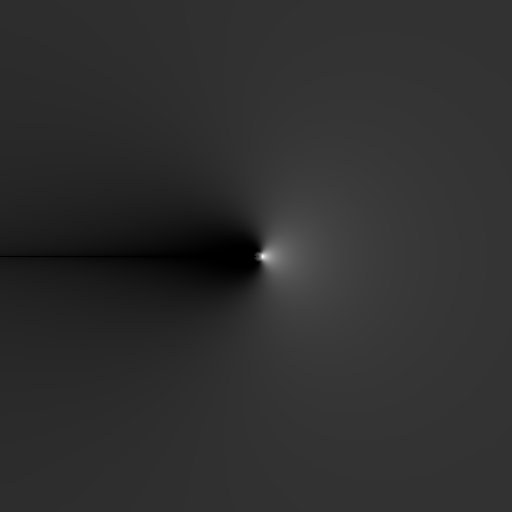
\includegraphics[scale=1]{figures/dfilt_wr_sqrt8.png}
 }
 \subbottom
 {
 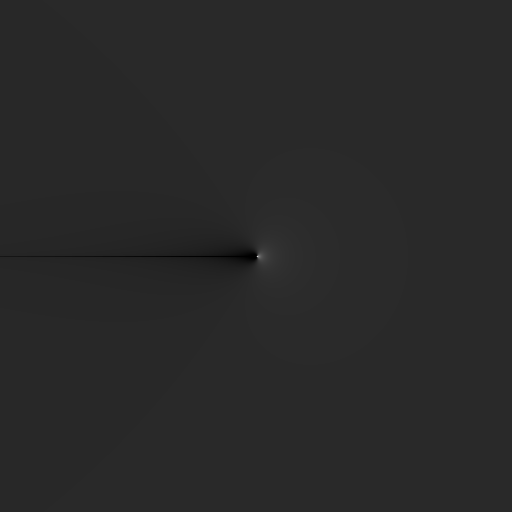
\includegraphics[scale=1]{figures/dfilt_wr_sqrt50.png}
 }
 \subbottom
 {
 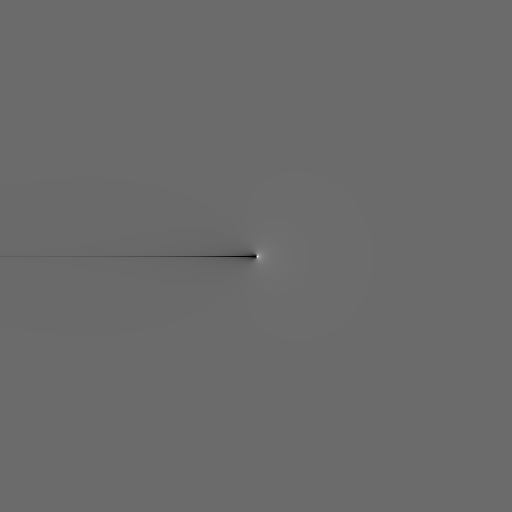
\includegraphics[scale=1]{figures/dfilt_wr_sqrt200.png}
 }
 \subbottom
 {
 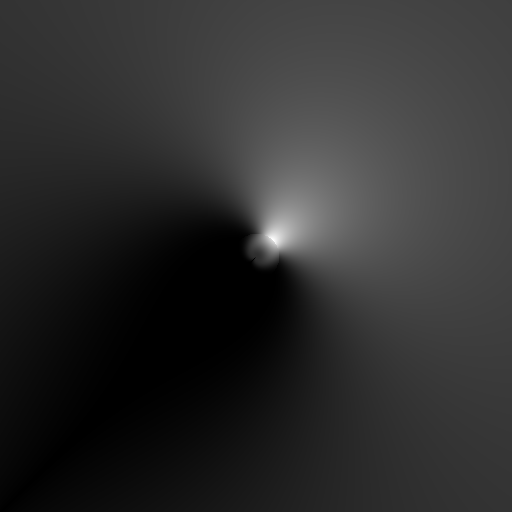
\includegraphics[scale=1]{figures/dfilt_wur_sqrt2.png}
 }
 \subbottom
 {
 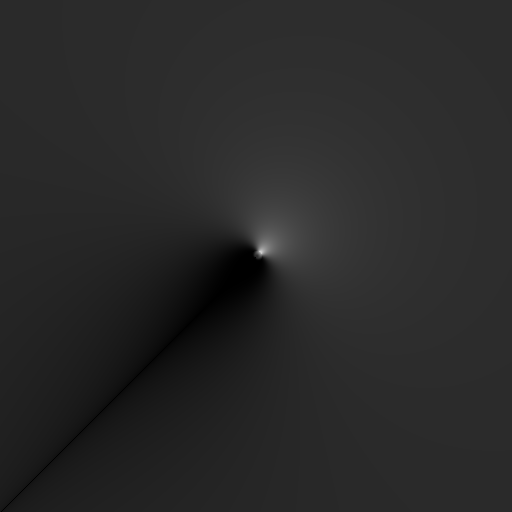
\includegraphics[scale=1]{figures/dfilt_wur_sqrt8.png}
 }
 \subbottom
 {
 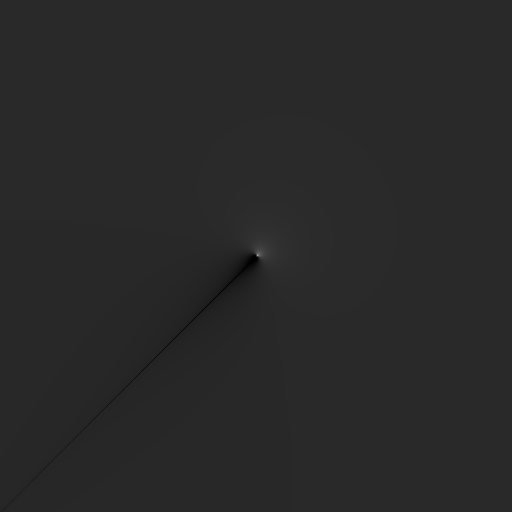
\includegraphics[scale=1]{figures/dfilt_wur_sqrt50.png}
 }
 \subbottom
 {
 
\includegraphics[scale=1]{figures/dfilt_wur_sqrt200.png}
 }
\caption{A set of instances of the directional spreading function, each column 
corresponds to a different wind speed, starting with the weakest one at the 
left. In the top row, the wind direction points to the right, in the bottom row 
to the upper right.}
\label{fig:directional_filter}
\end{figure}
%
Literature provides us with a large set of different directional spreading
functions to choose from. We picked a~\emph{Cosine-2s} variant based on the
work of Mitsuyasu et al.\cite{article:Mitsuyasu1975} and Hasselmann et 
al\cite{article:Hasselmann1980}. Expressed in terms of angular frequency 
$\omega$ it is as follows:
\begin{subequations}
\label{eq:directional_spread_mitsuyasu}
\begin{align}
 D(\omega, \theta) &=
\frac{2^{2s-1}}{\pi}~\frac{\Gamma^2(s+1)}{\Gamma(2s+1)}
~\left|\cos\left(\frac{\theta_{w}-\theta}{2}\right)\right|^{2s}
\intertext{with}
\frac{s}{s_p} &= \begin{cases}
(\frac{\omega}{\omega_p})^{-2.5} & \omega \geq \omega_p\\
(\frac{\omega}{\omega_p})^{5} & \omega < \omega_p\\
\end{cases}
\intertext{where, according to Hasselmann et al.}
s_p &= \begin{cases}
9.77 & \omega \geq \omega_p\\
6.97 & \omega < \omega_p\\
\end{cases}
\end{align}
\end{subequations}
$\Gamma$ is the \emph{gamma function}, $s$ is called the~\emph{spreading 
factor}, $\theta_w$ is the direction of the wind and $\omega_p$ represents the 
angular frequency the frequency spectrum has its peak at. 
Figure~\ref{fig:directional_filter} depicts example instances of 
Equation~\ref{eq:directional_spread_mitsuyasu}.
%
\subsection{Pierson Moskowitz Spectrum}
\label{sec:pierson_moskowitz}
%
% \begin{figure}
% \centering
% \begin{tikzpicture}
% \begin{axis}[
%     width=0.5\paperwidth,
%     legend style={draw=none},
%     xlabel={Frequency~$\omega$~($\text{rad}\cdot\text{s}^{-1}$)},
%     ylabel={Energy~$\Theta$~($\text{m}^2\cdot\text{s}$)},
%     every axis legend/.append style={nodes={right}},
%     ]
% 
% \addplot[
%     color=red,
%     solid,
% 	]
%     table [col sep=comma]{figures/pm_10.dat};
% \addlegendentry{$10.0~\text{m}\cdot\text{s}^{-1}$}
% \addplot[
%     color=green,
%     solid,
% 	]
%     table [col sep=comma]{figures/pm_12.dat};
% \addlegendentry{$12.5~\text{m}\cdot\text{s}^{-1}$}
% \addplot[
%     color=magenta,
%     solid,
% 	]
%     table [col sep=comma]{figures/pm_15.dat};
% \addlegendentry{$15.0~\text{m}\cdot\text{s}^{-1}$}
% \addplot[
%     color=black,
%     solid,
% 	]
%     table [col sep=comma]{figures/pm_17.dat};
% \addlegendentry{$17.5~\text{m}\cdot\text{s}^{-1}$}
% \addplot[
%     color=blue,
%     solid,
% 	]
%     table [col sep=comma]{figures/pm_20.dat};
% \addlegendentry{$20.0~\text{m}\cdot\text{s}^{-1}$}
% \end{axis}
% \end{tikzpicture}
% \caption{The Pierson Moskowitz frequency spectrum with different wind speed 
% values $U_{10}$.}
% \label{fig:pm_spectra}
% \end{figure}
\begin{figure}
\centering
\begin{tikzpicture}
\begin{groupplot}[
	group style={
		group size=2 by 1,
		xlabels at=edge bottom,
		ylabels at=edge left,
	},
    xlabel={Frequency~$\omega$~($\text{rad}\cdot\text{s}^{-1}$)},
    ylabel={Energy~$\Theta$~($\text{m}^2\cdot\text{s}$)},
	]
\nextgroupplot[
    legend style={draw=none},
    every axis legend/.append style={nodes={right}}
	]
\addplot[
    color=red,
    solid,
	]
    table [col sep=comma]{figures/pm_10.dat};
	\addlegendentry{$10.0~\text{m}\cdot\text{s}^{-1}$}
\addplot[
    color=green,
    solid,
	]
    table [col sep=comma]{figures/pm_12.dat};
	\addlegendentry{$12.5~\text{m}\cdot\text{s}^{-1}$}
\addplot[
    color=magenta,
    solid,
	]
    table [col sep=comma]{figures/pm_15.dat};
	\addlegendentry{$15.0~\text{m}\cdot\text{s}^{-1}$}
\addplot[
    color=black,
    solid,
	]
    table [col sep=comma]{figures/pm_17.dat};
	\addlegendentry{$17.5~\text{m}\cdot\text{s}^{-1}$}
\addplot[
    color=blue,
    solid,
	]
    table [col sep=comma]{figures/pm_20.dat};
	\addlegendentry{$20.0~\text{m}\cdot\text{s}^{-1}$}
\nextgroupplot[
    legend style={draw=none},
    every axis legend/.append style={nodes={right}}
	]
\addplot[
    color=magenta,
    solid,
	]
    table [col sep=comma]{figures/pm_15.dat};
	\addlegendentry{Unmodified}
\addplot[
    color=green,
    densely dashed,
	]
    table [col sep=comma]{figures/pm_15_alpha_07.dat};
	\addlegendentry{$\alpha \times 0.7$}
\addplot[
    color=blue,
    densely dashed,
	]
    table [col sep=comma]{figures/pm_15_alpha_12.dat};
	\addlegendentry{$\alpha \times 1.2$}
\addplot[
    color=black,
    dashdotted,
	]
    table [col sep=comma]{figures/pm_15_omegap_09.dat};
	\addlegendentry{$\omega_p \times 0.9$}
\addplot[
    color=red,
    dashdotted,
	]
    table [col sep=comma]{figures/pm_15_omegap_13.dat};
	\addlegendentry{$\omega_p \times 1.3$}
\end{groupplot}
\end{tikzpicture}
\caption{Left: The Pierson Moskowitz frequency spectrum with different wind 
speed values $U_{10}$. Right: Influence of the constant $\alpha$ and
the peak frequency $\omega_p$ on the resulting spectrum ($U_{10} = 
15.0~\text{m}\cdot\text{s}^{-1}$).}
\label{fig:pm_spectra}
\end{figure}
%
The Pierson Moskowitz spectrum~\cite{article:PiersonMoskowitz1964} is a well 
known and widely used one dimensional frequency spectrum. At the time it was 
introduced, it was expressed in terms of wind speed as follows:
\begin{subequations}
\label{eq:pierson_moskowitz_old}
\begin{align}
 \Theta(\omega) &= \frac{\alpha
g^2}{\omega^5}~\exp\left[-\beta\left(\frac{g}{U_{19.5}}\frac{1}{\omega}
\right)^4\right ]\\
\intertext{with}
\alpha &= 8.1 \times 10^{-3} \label{eq:pierson_moskowitz_alpha} \\
\beta &= 74 \times 10^{-1} \label{eq:pierson_moskowitz_beta}
\end{align}
\end{subequations}
where $U_{19.5}$ is the wind speed at a height of 19.5 meters above the sea
surface, the height of the anemometers used by Pierson and Moskowitz. Further
analysis of the data brought to light a relationship between wind speed and
peak frequency $\omega_p$
\begin{equation}
 \beta\left(\frac{g}{U_{19.5}}\right)^4 = \frac{5}{4}~\omega_p^4
\end{equation}
which lead to a rephrasing of Equation~\ref{eq:pierson_moskowitz_old} in terms
of peak frequency
\begin{subequations}
\label{eq:pierson_moskowitz}
\begin{gather}
 \Theta(\omega) = \frac{\alpha
g^2}{\omega^5}~\exp\left[-\frac{5}{4}\left(\frac{\omega_p}{\omega}
\right)^4\right ]\\
\intertext{with}
\omega_p = \sqrt[4]{\beta~\frac{4}{5}}~\frac{g}{U_{19.5}} \approx
0.877~\frac{g}{U_{19.5}}
\end{gather}
\end{subequations}
Most spectral models, which were published after the Pierson Moskowitz spectrum,
use wind speed at ten meters height above the sea surface, $U_{10}$, as a 
standard. We may convert between $U_{19.5}$ and $U_{10}$ as follows:
\begin{equation}
 U_{10} \approx 1.026\times U_{19.5}
\end{equation}
Now we are able to rewrite peak frequency $\omega_p$ in terms of $U_{10}$
\begin{equation}
 \omega_p \approx 0.855~\frac{g}{U_{10}}
\end{equation}
which completes our conversion of the Pierson Moskowitz model to standard wind 
speed $U_{10}$.\\

The proper use of the Pierson Moskowitz spectrum is restricted to~\emph{fully
developed seas}. A fully developed sea is a sea for which the energy input
to the waves from the wind is in equilibrium with the transfer of energy
among different wave components, and with the dissipation of energy by wave 
breaking. All wind generated waves are as large as they can be under the 
current conditions. Moreover, a fully developed sea is independent 
of~\emph{fetch}, which is the distance over which the wind blows, usually
limited by the upwind distance to shore.
%
%
\subsection{JONSWAP Spectrum}
\label{sec:jonswap}
%
The JONSWAP spectrum is one dimensional frequency spectrum  which has been 
developed by Hasselmann et al.\cite{article:Hasselman1973} based on data 
collected during the~\emph{Joint North Sea Wave Project}. The JONSWAP spectrum 
is expressed with the Pierson Moskowitz spectrum from 
Equation~\ref{eq:pierson_moskowitz} as basis, and an additional peak factor:
%
\begin{subequations}
\begin{gather}
 \Theta(\omega) = \frac{\alpha
g^2}{\omega^5}~\exp\left[-\frac{5}{4}\left(\frac{\omega_p}{\omega}
\right)^4\right]\gamma^r\\
\intertext{with}
r = \exp\left[-\frac{\left(\omega -
\omega_p\right)^2}{2\sigma^2\omega_p^2}\right] \\
\alpha = 0.076\left(\frac{U_{10}^2}{Fg}\right)^{0.22} \\
\omega_{p} = 22\left(\frac{g^2}{U_{10}F}\right)^{1/3} \\
\sigma = \begin{cases}
	0.07 & \omega\leq\omega_p\\
	0.09 & \omega > \omega_p
    \end{cases} \\
\gamma = 3.3
\end{gather}
\end{subequations}
where $F$ denotes the fetch in centimeters and $U_{10}$ the wind speed in 
meters per second at a height of 10 meters above the sea surface.\\

%
\begin{figure}
\centering
\subtop[Wind speed $U_{10} = 15m\cdot s^{-1}$]
{
\label{subfig:jonswap_spectra_15}
\begin{tikzpicture}
\begin{axis}[
    width=0.7\textwidth,
    xlabel={Frequency~$\omega$~($\text{rad}\cdot\text{s}^{-1}$)},
    ylabel={Energy~$\Theta$~($\text{m}^2\cdot\text{s}$)},
    legend to name=jonswap_fetches_legend,
    legend columns=-1,
    ]
\addplot[
    color=blue,
    solid,
    ]
    table [col sep=comma]{figures/pm_15.dat};
\addlegendentry{Pierson Moskowitz}
\addplot[
    color=red,
    solid,
    ]
    table [col sep=comma]{figures/j_15_100km.dat};
\addlegendentry{100km}
\addplot[
    color=green,
    solid,
    ]
    table [col sep=comma]{figures/j_15_200km.dat};
\addlegendentry{200km}
\addplot[
    color=magenta,
    solid,
    ]
    table [col sep=comma]{figures/j_15_300km.dat};
\addlegendentry{300km}
\addplot[
    color=black,
    solid,
    ]
    table [col sep=comma]{figures/j_15_400km.dat};
\addlegendentry{400km}
\end{axis}
\end{tikzpicture}
}
\subtop[Wind speed $U_{10} = 10m\cdot s^{-1}$]
{
\label{subfig:jonswap_spectra_10}
\begin{tikzpicture}
\begin{axis}[
    width=0.7\textwidth,
    xlabel={Frequency~$\omega$~($\text{rad}\cdot\text{s}^{-1}$)},
    ylabel={Energy~$\Theta$~($\text{m}^2\cdot\text{s}$)},
    ]
\addplot[
    color=blue,
    solid,
    ]
    table [col sep=comma]{figures/pm_10.dat};
\addplot[
    color=red,
    solid,
    ]
    table [col sep=comma]{figures/j_10_100km.dat};
\addplot[
    color=green,
    solid,
    ]
    table [col sep=comma]{figures/j_10_200km.dat};
\addplot[
    color=magenta,
    solid,
    ]
    table [col sep=comma]{figures/j_10_300km.dat};
\addplot[
    color=black,
    solid,
    ]
    table [col sep=comma]{figures/j_10_400km.dat};
\end{axis}
\end{tikzpicture}
}
\ref{jonswap_fetches_legend}
\caption{JONSWAP frequency spectra with different fetch values $F$. Note the more
and more pronounced peak of the JONSWAP spectrum as fetch increases. Moreover,
the frequency range the  peak of the JONSWAP spectrum lies in, tends towards
lower frequencies as fetch increases.}
\label{fig:jonswap_spectra_fetches}
\end{figure}
%
Hasselmann et al. found that in context of their model the sea is actually 
never fully developed, the  spectrum does not converge to the basic Pierson 
Moskowitz spectrum as fetch increases. Said effect is discussed at 
length by Hasselmann et al. and in the end attributed to non-linear wave-wave 
interactions. Figure~\ref{fig:jonswap_spectra_fetches} gives a tentative 
overview of the development of a JONSWAP modeled sea as fetch increases, 
including a Pierson Moskowitz spectrum for comparison. One may see that the 
spectral peak of the JONSWAP spectrum may take a more narrow form than the 
already pronounced peak of the Pierson Moskowitz spectrum, see
Figure~\ref{subfig:jonswap_spectra_15}. Moreover, with increasing fetch, said
peak may move to an even lower frequency range than its Pierson Moskowitz
counterpart, see Figure~\ref{subfig:jonswap_spectra_10}.
%
\subsection{Integral Domain Conversion}
%
\begin{figure}
\centering
\begin{tikzpicture}
\begin{axis}[
    width=0.5\paperwidth,
    scaled ticks=false,
    xticklabel style={/pgf/number format/fixed},
    xlabel={Wave number $k$~($\text{m}^{-1}$)},
    ylabel={Energy~$\Theta$~($\text{m}^2$)},
    legend style={draw=none},
    every axis legend/.append style={nodes={right}},
    ]
\addplot[
    color=blue,
    solid,
	]
    table [col sep=comma]{figures/pm_15_k.dat};
\addlegendentry{Pierson Moskowitz}
\addplot[
    color=red,
    solid,
	]
    table [col sep=comma]{figures/j_15_100km_k.dat};
\addlegendentry{100km}
\addplot[
    color=green,
    solid,
	]
    table [col sep=comma]{figures/j_15_200km_k.dat};
\addlegendentry{200km}
\addplot[
    color=magenta,
    solid,
	]
    table [col sep=comma]{figures/j_15_300km_k.dat};
\addlegendentry{300km}
\addplot[
    color=black,
    solid,
	]
    table [col sep=comma]{figures/j_15_400km_k.dat};
\addlegendentry{400km}
\end{axis}
\end{tikzpicture}
\caption{Pierson Moskowitz and JONSWAP frequency spectra
$\Theta_{\omega}(\omega$) from Figure~\ref{subfig:jonswap_spectra_15}
converted into one dimensional wave number spectra $\Theta_k(k)$.}
\label{fig:jonswap_spectra_fetches_k}
\end{figure}
%
% \begin{figure}
% \centering
% \begin{tikzpicture}
% \begin{groupplot}[
%   group style={
%     group size=2 by 1,
% %    horizontal sep=2cm
%   },
% ]
% \nextgroupplot[
%     width=0.5\textwidth,
%     scaled ticks=false,
%     xticklabel style={/pgf/number format/fixed},
%     xlabel={Frequency~$\omega$~($\text{rad}\cdot\text{s}^{-1}$)},
%     ylabel={Energy~$\Theta$~($\text{m}^2\cdot\text{s}$)},
%     legend to name=brak_legend,
%     legend columns=-1,
%     legend style={draw=none, /tikz/every even column/.append 
% style={column sep=0.25cm}},
% ]
% \addplot[
%     color=blue,
%     solid,
%     ]
%     table [col sep=comma]{figures/pm_15.dat};
% \addlegendentry{Pierson Moskowitz}
% \addplot[
%     color=red,
%     solid,
%     ]
%     table [col sep=comma]{figures/j_15_100km.dat};
% \addlegendentry{100km}
% \addplot[
%     color=green,
%     solid,
%     ]
%     table [col sep=comma]{figures/j_15_200km.dat};
% \addlegendentry{200km}
% \addplot[
%     color=magenta,
%     solid,
%     ]
%     table [col sep=comma]{figures/j_15_300km.dat};
% \addlegendentry{300km}
% \addplot[
%     color=black,
%     solid,
%     ]
%     table [col sep=comma]{figures/j_15_400km.dat};
% \addlegendentry{400km}
% 
% \nextgroupplot[
%     width=0.5\textwidth,
%     scaled ticks=false,
%     xticklabel style={/pgf/number format/fixed},
%     xlabel={Wave number $k$~($\text{m}^{-1}$)},
%     ylabel={Energy~$\Theta$~($\text{m}^2$)},
%     ytick pos=right,
% ]
% \addplot[
%     color=blue,
%     solid,
% 	]
%     table [col sep=comma]{figures/pm_15_k.dat};
% \addplot[
%     color=red,
%     solid,
% 	]
%     table [col sep=comma]{figures/j_15_100km_k.dat};
% \addplot[
%     color=green,
%     solid,
% 	]
%     table [col sep=comma]{figures/j_15_200km_k.dat};
% \addplot[
%     color=magenta,
%     solid,
% 	]
%     table [col sep=comma]{figures/j_15_300km_k.dat};
% \addplot[
%     color=black,
%     solid,
% 	]
%     table [col sep=comma]{figures/j_15_400km_k.dat};
% \end{groupplot}
% %\node at (plots c1r1.north) [anchor=south, yshift=.6cm] {\ref{brak_legend}};
% \node (l1) at ($(group c1r1.south)!0.5!(group c2r1.south)$)
%       [below, yshift=-3\pgfkeysvalueof{/pgfplots/every axis title shift}]
%       {\ref{brak_legend}};
% \end{tikzpicture}
% \caption{BRAK.}
% \end{figure}
%
Recall that we transform from the cartesian wave number domain to the spatial 
one. Thus, as a prerequisite, we are in need of a two dimensional wave number 
spectrum $\Theta(\mvec{k})$, but 
Equation~\ref{eq:directional_frequency_spectrum} 
gives us a directional frequency spectrum $\Theta(\omega,\theta)$. We will 
convert one spectrum form to the other according to the substitution rule, with 
the deep water dispersion relation from Equation~\ref{eq:disp_rel_deep_water} 
serving as a link between angular frequency $\omega$ and wave number $k$. To 
avoid possible confusion we will add subscripts to each occurence of $\Theta$ 
in order to explicitely show the parameters it takes as input.\\

As a first step we may transform the one dimensional frequency spectrum 
$\Theta_{\omega}(\omega)$ to the one dimensional wave number 
spectrum $\Theta_k(k)$ as follows:
\begin{subequations}
\begin{multline}
 \int\Theta_k(k)~\mathrm{d}k = \int\Theta_{\omega}(\omega)~\mathrm{d}\omega\\ = 
\int\Theta_{\omega}(\omega(k))\frac{\mathrm{d}\omega}{\mathrm{d}k}~\mathrm{d}k
= \int\Theta_{\omega}(\sqrt{gk})\frac{1}{2}\sqrt{\frac{g}{k}}~\mathrm{d}k
\end{multline}
which gives us
\begin{equation}
\label{eq:theta_k}
 \Theta_k(k) = \Theta_{\omega}(\sqrt{gk})\frac{1}{2}\sqrt{\frac{g}{k}}
\end{equation}
\end{subequations}
%
A set of one dimensional wave spectra $\Theta_k(k)$ may be seen in
Figure~\ref{fig:jonswap_spectra_fetches_k}. Note the difference in scale on the ordinate
in comparison to the one dimensional frequency spectra $\Theta_{\omega}(\omega)$
depicted in Figure~\ref{fig:jonswap_spectra_fetches}.\\

%
\begin{figure}
\centering
\subbottom
{
\label{sfig:polar}
\begin{tikzpicture}
\begin{axis}[
    width=0.5\paperwidth,
    view={-20}{30},
    mesh/ordering=y varies,
    zlabel={Energy~$\Theta$~($\text{m}^2\cdot\text{s}$)},
    xlabel={Frequency~$\omega$~($\text{rad}\cdot\text{s}^{-1}$)},
    ylabel={Direction~$\theta$~($\text{rad}$)},
    ]
\addplot3[surf,
    ]
    table [col sep=comma]{figures/jonswap_w15_f100_omega_angle.dat};
\end{axis}
\end{tikzpicture}
}
\subbottom
{
\label{sfig:wave_vector}
\begin{tikzpicture}
\begin{axis}[
    width=0.5\paperwidth,
    view={-20}{30},
    mesh/ordering=y varies,
    xtick = {0,0.1,0.2},
    zlabel={Energy~$\Theta$~($\text{m}^4$)},
    xlabel={$k_x$~($\text{m}^{-1}$)},
    ylabel={$k_y$~($\text{m}^{-1}$)},
    ]
\addplot3[surf,
    ]
    table [col sep=comma]{figures/jonswap_w15_f100_kx_ky.dat};
\end{axis}
\end{tikzpicture}
}
\caption{The JONSWAP frequency spectrum with wind speed $U_{10} = 15m\cdot 
s^{-1}$ and fetch $F = 100km$, located in two different domains. Top: the polar
coordinate domain $\omega \times \theta$, the wind direction points in the
direction of the positive $\omega$ axis. Bottom: the wave vector domain
$k_x \times k_y$, the wind direction points in the direction of the positive
$k_x$ axis. Note the difference in scale between the two vertical axes.}
\label{fig:jonswap_3d_omega_theta_kx_ky}
\end{figure}
%
Given $\Theta_k(k)$ we are able to rewrite the directional frequency spectrum
$\Theta_{\omega, \theta}(\omega, \theta)$ from
Equation~\ref{eq:directional_frequency_spectrum} in terms of wave number $k$:
%
\begin{equation}
\label{eq:theta_k_polar}
 \Theta_{k,\theta}(k,\theta) = \Theta_k(k)D(\sqrt{gk},\theta)
\end{equation}
%
where $\Theta_{k,\theta}(k,\theta)$ is called the~\emph{directional wave number 
spectrum}. As the last step we need to convert from polar coordinate pairs 
$(k,\theta)$ to cartesian wave number coordinates $\mvec{k}$. Said conversion 
is accomplished as follows:
%
\begin{equation}
\label{eq:theta_cart_to_polar}
\int\Theta_{\mvec{k}}(\mvec{k})~\mathrm{d}\mvec{k} = 
\int\int\Theta_{k,\theta}(k,\theta)\frac{1}{k}~\mathrm{d}\theta~\mathrm{d}k
\end{equation}
%
By combining Equations~\ref{eq:directional_frequency_spectrum}, 
~\ref{eq:theta_k} and~\ref{eq:theta_cart_to_polar} we get the Cartesian wave 
number spectrum:
%
\begin{align}
\Theta_{\mvec{k}}(\mvec{k}) &= \Theta_{\omega,\theta}(\sqrt{gk}, 
\theta)\frac{1}{2k}\sqrt{\frac{g}{k}}\\
\intertext{where}
\theta &= \arctan\left(\frac{k_y}{k_x}\right)
\end{align}
%
An instance of a directional frequency spectrum as well as its equivalent
directional wave number spectrum are depicted in Figure
\ref{fig:jonswap_3d_omega_theta_kx_ky}.\\

Now we are able to preserve integral equality between different representations 
of $\Theta$, as long as we use the deep water dispersion relation. One may do 
the math for another dispersion relation, now that the path to walk is laid 
out. Still, in the context of this work, we only concern ourselves with waves 
in deep water.
%
\section{Two dimensional Frequency Spectra}

\subsection{Phillips Spectrum}
\label{sec:phillips_spectrum}
%
The Phillips Spectrum, as introduced by Tessendorf~\cite{course:simulatingocean}, is an ad-hoc formulation of a two dimensional wave number spectrum $\Theta(\mvec{k})$. It has been developed with computer graphic purposes in mind, and as such it lacks a solid oceanographic foundation. We may write Tessendorf's formulation of the Phillips Spectrum in a manner consistent with our notation as follows:
%
\begin{subequations}
\begin{gather}
\label{eq:phillips_spectrum}
 \Theta(\mvec{k}) = A\frac{\exp\left(-(kL)^{-2}-(kl)^2\right)}{k^4}\abs*{\transpose{\mvec{k}_n}\mvec{w}_n}^2\\
\intertext{with}
\mvec{k}_n = \frac{\mvec{k}}{\norm{\mvec{k}}} = \frac{\mvec{k}}{k}\\
\mvec{w}_n = \frac{\mvec{w}}{\norm{\mvec{w}}}\\
L = \frac{\norm{\mvec{w}}^2}{g}
\end{gather}
\end{subequations}
%
where $A$ and $l$ are numeric constants, and $\mvec{w}$ encodes wind 
direction and wind speed $\norm{\mvec{w}}$. The numeric constant $A$ represents 
a scaling factor which we will discuss at a later point.  According to 
Tessendorf~\cite{course:simulatingocean}, $L$ defines the largest possible wave
arising from a continuous wind of speed $\norm{\mvec{w}}$. The parameter $l$ on 
the other hand acts as a frequency filter, it is meant to make the suppression 
of energy contributed by high wave numbers $k$ possible. In order to do that it 
is mandatory for $l$ to be several orders of magnitude smaller than $L$. We 
chose the following as a default value for $l$:
\begin{equation}
 l = 10^{-3}L
\end{equation}
Moreover, one may conclude from Equation~\ref{eq:phillips_spectrum} that setting 
$l = 0$ disables any wave number based suppression of energy.\\

If we take a closer look at Equation~\ref{eq:phillips_spectrum} one may notice 
similarities to a one dimensional frequency spectrum in combination with a 
directional spread as seen in Equation~\ref{eq:directional_frequency_spectrum}. 
We may separate the terms involved as follows:
\begin{equation}
\label{eq:phillips_spectrum_separated}
 \Theta(\mvec{k}) = \underbrace{A}_{Scale}\underbrace{\frac{\exp\left(-(kL)^{-2}-(kl)^2\right)}{k^4}}_{\substack{one~dimensional\\wave~ number\\spectrum}}\underbrace{\abs*{\transpose{\mvec{k}_n}\mvec{w}_n}^2}_{\substack{directional\\spread}}
\end{equation}
%
\begin{figure}
\centering
\begin{tikzpicture}
\begin{axis}[
    width=0.5\paperwidth,
    legend style={draw=none},
    xlabel={Wave number~$k$~($\text{m}^{-1}$)},
    ylabel={Energy~$\Theta$},
    scaled ticks=false,
    xticklabel style={/pgf/number format/fixed},
    every axis legend/.append style={nodes={right}},
    ]

\addplot[
    color=red,
    solid,
	]
    table [col sep=comma]{figures/phillips_10.dat};
\addlegendentry{$10.0~\text{m}\cdot\text{s}^{-1}$}
\addplot[
    color=green,
    solid,
	]
    table [col sep=comma]{figures/phillips_12.dat};
\addlegendentry{$12.5~\text{m}\cdot\text{s}^{-1}$}
\addplot[
    color=magenta,
    solid,
	]
    table [col sep=comma]{figures/phillips_15.dat};
\addlegendentry{$15.0~\text{m}\cdot\text{s}^{-1}$}
\addplot[
    color=black,
    solid,
	]
    table [col sep=comma]{figures/phillips_17.dat};
\addlegendentry{$17.5~\text{m}\cdot\text{s}^{-1}$}
\addplot[
    color=blue,
    solid,
	]
    table [col sep=comma]{figures/phillips_20.dat};
\addlegendentry{$20.0~\text{m}\cdot\text{s}^{-1}$}
\end{axis}
\end{tikzpicture}
\caption{The one dimensional wave number spectrum term of the Phillips 
frequency spectrum with different wind speed values $\norm{\mvec{w}}$. The shape 
of the spectrum resembles the Pierson Moskowitz spectrum, the scale on the 
other hand differs at least by a magnitude of $10^4$.}
\label{fig:phillips_spectra}
\end{figure}
%
A set of instances of the one dimensional wave number spectrum term is depicted 
in Figure~\ref{fig:phillips_spectra}. One may see that the shape of the 
spectrum is similar to the Pierson Moskowitz one in Figure~\ref{fig:pm_spectra}, 
with the frequency range of the spectrum peak being located at even lower 
frequencies than the Pierson Moskowitz and JONSWAP ones. The magnitude of the 
energy on the other hand exceeds the one given by Pierson Moskowitz and JONWAP 
by at least a factor of $10^4$. Recall that both the Pierson Moskowitz and the 
JONSWAP model are based on real world data aquired on the ocean, then we may 
reason that those models give us a value range for energy precise enough to 
generate believable results. Therefore we need to rescale the energy obtained 
from the Phillips spectrum into that range. To the author it seems reasonable 
that that is the purpose of the numeric constant $A$ in 
Equations~\ref{eq:phillips_spectrum} and \ref{eq:phillips_spectrum_separated}. 
Since Tessendorf does not give any information about $A$, choosing a value that 
scales energy appropriately for all reasonable input parametrisations has proven 
to be difficult. The constant $\alpha = 8.1 \times 10^{-3}$ from Equation
\ref{eq:pierson_moskowitz_old} seemed to be promising initially, but in the end 
the author settled for the following more complex solution:
\begin{align}
 A = \frac{0.81}{LK}B && B \in \interval{0}{1}
\end{align}
where $L$ and $K$ represent side lengths in meters of the rectangular area 
we want to synthesize.
%
\begin{figure}
 \centering
 \subbottom[$\cos^2$]
 {
 \label{subfig:directional_spread_cos2_r}
 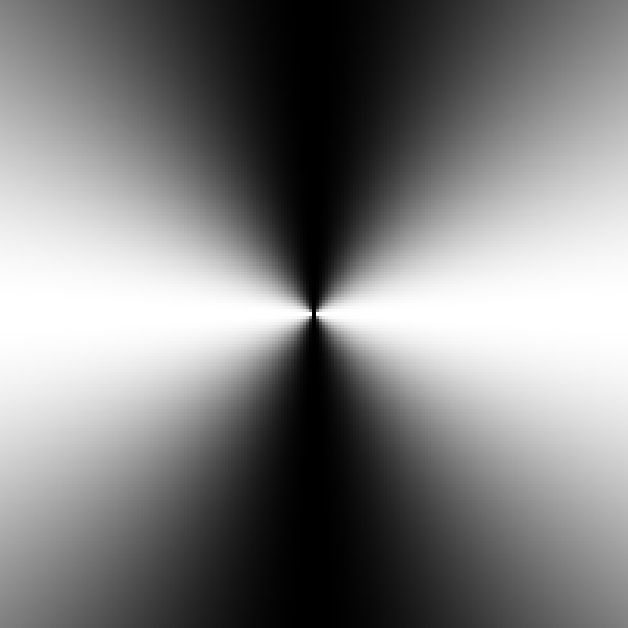
\includegraphics[scale=0.6]{figures/phillips_dir_r_exponent_2.png}
 }
 \subbottom[$\cos^4$]
 {
\label{subfig:directional_spread_cos4_r}
 
\includegraphics[scale=0.6]{figures/phillips_dir_r_exponent_4.png}
 }
 \subbottom[$\cos^2$]
 {
 \label{subfig:directional_spread_cos2_ur}
 
\includegraphics[scale=0.6]{figures/phillips_dir_ur_exponent_2.png}
 }
 \subbottom[$\cos^4$]
 {
 \label{subfig:directional_spread_cos4_ur}
 
\includegraphics[scale=0.6]{figures/phillips_dir_ur_exponent_4.png}
 }
\caption{Example instances of the Phillips directional spreading function with 
exponents $2$ and $4$. For~\subcaptionref{subfig:directional_spread_cos2_r} and
\subcaptionref{subfig:directional_spread_cos4_r} the wind direction poins to 
the right, for \subcaptionref{subfig:directional_spread_cos2_ur} and
\subcaptionref{subfig:directional_spread_cos4_ur} it points to the upper right. 
The directional spread with an exponent equal $4$ is distinctly more narrow 
than the one with an exponent equal $2$. Moreover, all instances have an easy 
to identify symmetry axis.}
\label{fig:phillips_directional_term}
\end{figure}
%
Now that we have discussed the one dimensional wave number spectrum and the 
scale factor $A$, we move on to the directional term from 
Equation~\ref{eq:phillips_spectrum_separated}. Said term is a simple cosinus 
term raised to the power of two, with normalised wave vector $\mvec{k}$ and 
normalised wind vector $\mvec{w}$ as input. We may increase the exponent in 
order to make the resulting directional spread more narrow. Moreover, since 
only the absolute value of the cosinus is taken into account, results for 
$\mvec{k}$ and $-\mvec{k}$ are the same. A direct consequence is a symmetry not 
only of the directional spread but of the entire Phillips spectrum: 
$\Theta(\mvec{k}) = \Theta(-\mvec{k})$. Figure 
\ref{fig:phillips_directional_term} gives an illustration of the directional 
spread with different wind directions and different exponents. Recall that the 
directional spread $D$ distributes the energy represented by $\Theta(k)$ among 
all directions, without changing the amount of energy at wave number $k$.  
Energy is conserved, therefore we may write similar to Section 
\ref{sec:1d_frequency_spectra}:
\begin{subequations}
\begin{align}
\int_{\theta=-\pi}^{\pi}D(\sqrt{gk},\theta)~\mathrm{d}\theta &= 1 \\
D(\sqrt{gk},\theta) &\geq 0
\end{align}
\end{subequations}
We insert two variants of the Phillips directional spread into the integral:
\begin{subequations}
\begin{align}
\int_{\theta=-\pi}^{\pi} \abs{\cos(\theta)}^2~\mathrm{d}\theta &= \pi \\
\int_{\theta=-\pi}^{\pi} \abs{\cos(\theta)}^4~\mathrm{d}\theta &= \frac{3\pi}{4}
\end{align}
\end{subequations}
As one can see, the results are \emph{not} equal one, therefore energy is 
\emph{not} conserved. In combination with the unusual magnitude of energy 
output by the one dimensional Phillips wave number spectrum, it is really 
difficult to find an appropriate scale factor $A$ in order to generate 
believable ocean surfaces with the Phillips spectrum as basis.
%
\subsection{Unified Spectrum}
\label{sec_unified_spectrum}

\section{The Projected Grid}
\label{sec_projected_grid}
The projected grid is based on a simple concept: in order to achieve an
uniform distribution of details on the image plane, a uniformly spaced grid is
created in post-perspective space and transformed back to world space.
Figure~\ref{fig:projectedgrid} illustrates the difference between a classic
world space approach and the projected grid.
\begin{figure}[h]
\centering
\subbottom[Classic]
{
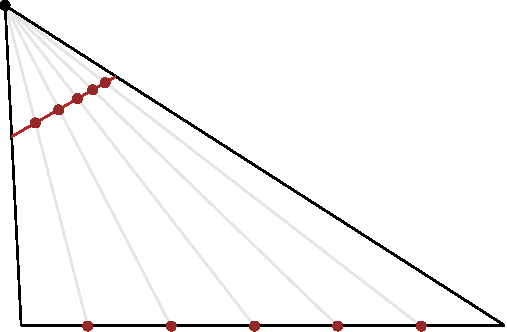
\includegraphics[scale=0.75]{figures/ProjectedGridVsWorldSpace.pdf}
\label{fig:subfigprojgrid1}
}
\subbottom[Projected Grid]
{
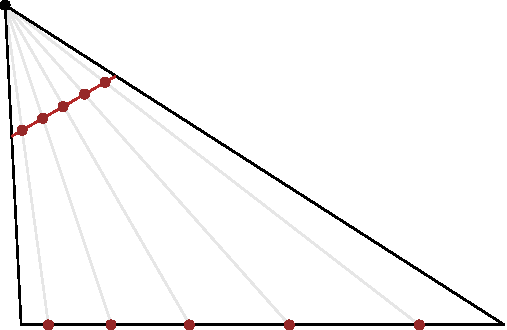
\includegraphics[scale=0.75]{figures/ProjectedGridUniform.pdf}
\label{fig:subfigprojgrid2}
}
\caption{The image on the left shows an uniform grid in worldspace,
its projection onto the image plane is not uniformly spaced though.
The image on the right on the other hand depicts an uniform grid on
the image plane and its associated non-uniform spaced worldspace
positions.}
\label{fig:projectedgrid}
\end{figure}

% The algorithm used for the projected grid can be broken down into the following
% steps:
% \begin{itemize}
%  \item create a uniformly spaced grid orthogonal to the viewer using normalised
% device coordinates
%  \item transform the grid to worldspace
%  \item project the grid onto the desired base plane
%  \item apply height displacement
%  \item run the grid through the rendering pipeline as usual
% \end{itemize}

\subsection{Coordinate Systems}
\label{sec:coordinate_systems}
Let $\mvec{x}$ be a vector representing the three dimensional carthesian
world space coordinate of a vertex, then
\begin{equation}
 \mvec{w} = \transpose{(\mvecx{x}, \mvecy{x}, \mvecz{x}, 1)}
\end{equation}
where $\mvec{w}$ is a homogeneous world space coordinate of $\mvec{x}$.
Let $\mmat{V}$ be the view matrix and $\mmat{P}$ the projection matrix, then
\begin{equation}
\label{eq:ws_to_cs}
 \mvec{c} = \mmat{P} \mmat{V} \mvec{w}
\end{equation}
where $\mvec{c}$ is the \textit{clip space} coordinate of $\mvec{w}$. For $\mvec{c}$ to
be inside the view frustum defined by $\mmat{P}$, $\mvec{c}$ is required to
meet the following condition
\begin{equation}
\label{eq:cs_bounds}
 \mvecx{c}, \mvecy{c}, \mvecz{c} \in \interval{-\mvecw{c}}{\mvecw{c}}
\end{equation}
where $\mvecw{c}$ is the homogeneous component of $\mvec{c}$. Next, clip space
vertex $\mvec{c}$ is transformed by the \textit{perspective division} as follows
\begin{equation}
\label{eq:cs_to_ndc}
 \mvec{n} = \frac{1}{\mvecw{c}}\transpose{(\mvecx{c}, \mvecy{c}, \mvecz{c})}
\end{equation}
where $\mvec{n}$ corresponds to the \textit{normalised device coordinate},
\textit{NDC} in short, of $\mvec{c}$.
%
%
\begin{figure}
\centering
\subbottom[View Frustum]
{
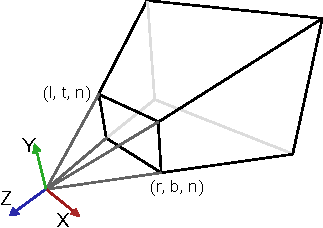
\includegraphics[width=0.4\textwidth]{figures/ProjectiveFrustum.pdf}
\label{fig:subfig_proj_frustum}
}
\subbottom[Canonical view volume]
{
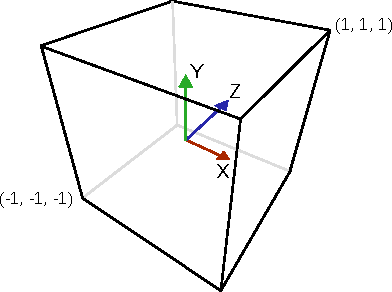
\includegraphics[width=0.4\textwidth]{figures/CanonicalCube.pdf}
\label{fig:subfig_canonical_view_volume}
}
\caption{Left: An example view frustum in view space. Right: The same view frustum
after applying projection and perspective division.}
\label{fig:proj_frustum_ndc}
\end{figure}
%
%
As one can see, equations~\ref{eq:cs_bounds}
and~\ref{eq:cs_to_ndc} imply
\begin{equation}
\label{eq:ndc_bounds}
 \mvecx{n}, \mvecy{n}, \mvecz{n} \in \interval{-1}{1}
\end{equation}
which defines the space NDC reside in, namely the \textit{canonical view volume},
see Figure~\ref{fig:proj_frustum_ndc}.\\


The projected grid, on the other hand, starts inside the canonical view volume
and needs to transform vertices back to world space. Let $\mvec{n}$ be the
normalised device coordinate of a vertex, then
\begin{equation}
\label{eq:ndc_to_cs}
 \mvec{c} = \transpose{(\mvecx{n}, \mvecy{n}, \mvecz{n}, 1)}
\end{equation}
where $\mvec{c}$ is a valid representation of $\mvec{n}$ in clip space. One may choose
a value for $\mvecw{c}$ different from $1$, making it necessary to scale $\mvecx{n}$,
$\mvecy{n}$ and $\mvecz{n}$ accordingly. Again, let $\mmat{V}$ be the view matrix and
$\mmat{P}$ the projection matrix, then
\begin{equation}
\label{eq:cs_to_wsh}
 \mvec{w} = \inverse{(\mmat{P} \mmat{V})} \mvec{c}
\end{equation}
where $\mvec{w}$ is a homogeneous world space coordinate of $\mvec{c}$. Conversion
to three dimensional carthesian world space is accomplished as follows
\begin{equation}
\label{eq:wsh_to_ws}
 \mvec{x} = \frac{1}{\mvecw{w}}\transpose{(\mvecx{w}, \mvecy{w}, \mvecz{w})}
\end{equation}

\subsection{Projection onto Plane}
As noted before, the vertices of the projected grid are represented as normalised
device coordinates. Assuming the plane the grid shall be projected on is specified
in world space coordinates, the following steps need to be computed for each vertex:
\begin{itemize}
 \item Transform vertex from canonical view volume to world space
 \item Setup vertex specific ray
 \item Intersect ray with target plane to compute actual position
\end{itemize}
Step one is already covered by Section~\ref{sec:coordinate_systems}. Step two
requires to setup a ray for each vertex, which implies both a position and a
direction. The position we already have, but to create a direction we need two
different positions. The solution is rather straightforward: let $\mvec{n}$ be
a \textit{two dimensional} vector representing the \textit{X} and \textit{Y}
components of a position in normalised device coordinates, then
\begin{align}
 \mvec{a} & = (\mvecx{n}, \mvecy{n}, -1, 1)\\
 \mvec{b} & = (\mvecx{n}, \mvecy{n}, +1, 1)
\end{align}
where $\mvec{a}$ corresponds to $\mvec{n}$ on the \textit{near plane} in clip space,
and $\mvec{b}$ to $\mvec{n}$ on the \textit{far plane} in clip space. Let $\mvec{d}$
and $\mvec{e}$ be the carthesian world space positions of $\mvec{a}$ and $\mvec{b}$
respectively, then
\begin{equation}
 \label{eq:proj_grid_ray}
 \mvec{p} = \mvec{d} + t(\mvec{e} - \mvec{d})
\end{equation}
where $\mvec{p}$ represents a ray starting at point $\mvec{d}$, pointing in direction
$(\mvec{e} - \mvec{d})$ with variable parameter $t$ controlling the actual position on
the ray.\\

Step three is about intersecting ray $\mvec{p}$ resulting from step two with the target plane.
We define the target plane using the \textit{Hesse normal form} as follows
\begin{equation}
\label{eq:proj_grid_plane}
 \mvec{p}\transpose{\mvec{n}} - d = 0
\end{equation}
where $\mvec{n}$ is the plane's normal vector with unit length and $d$ the plane's distance
from the origin. Next, we insert $\mvec{p}$ from equation~\ref{eq:proj_grid_ray}
into equation~\ref{eq:proj_grid_plane}, resulting in
%
\begin{gather}
\label{eq:plane_and_ray_intersection}
(\mvec{d} + t(\mvec{e} - \mvec{d})\transpose{\mvec{n}} - d = 0\\
\mvec{d}\transpose{\mvec{n}} + t(\mvec{e} - \mvec{d})\transpose{\mvec{n}} - d = 0\\
\intertext{solve for $t$}
t = \cfrac{d - \mvec{d}\transpose{\mvec{n}}}{(\mvec{e} - \mvec{d})\transpose{\mvec{n}}}
\end{gather}
%
where $t$ in combination with equation~\ref{eq:proj_grid_ray} gives the point of intersection
between the ray and the plane. In case $(\mvec{e} - \mvec{d})\transpose{\mvec{n}} = 0$,
there is no point of intersection because the ray is parallel to the plane.

\subsection{Projector}
\fxnote*{JÖSSAS}{Backfiring, etc}